\subsection{Drivetrain}\label{Drivetrain}

%% INTRODUCTION %%
The drivetrain translates the torque $\tau_m$, given by the motor, into the actual movement of the vehicle. The model of the drivetrain illustrates the relation between the applied torque, $\tau_m$, and the velocity of the vehicle. The velocity model of the drivetrain is created by only considering when the vehicle's trajectory follows a straight line.\\\\
%
The modelling of the drivetrain is limited to only model parts of the total drivetrain system, to make it more manageable and with a focus on giving a rough approximation.
%% SSSECTION : BLACK BOX MODEL %%
\subsubsection{Black Box Model}\label{BlackBoxModel}
To get a rough approximation of how the drivetrain works, a blackboxed model is used. The blackbox in the model is placed between box 1 and including box 4 seen in \chapref{VehicleDescription} \figref{vehicleDescriptionDriveTrain}. The gear, $G_m$, connected to the motor shaft, is connected to the gear ,$G_d$, which represents the gears and shaft that has been black boxed and the drive-wheel, see \figref{fig:DrivetrainMechanicalModel}. The number of teeth on the gear, $G_d$, is set to the total gear ratio of the black box.

\begin{figure}[H]
	\centering
	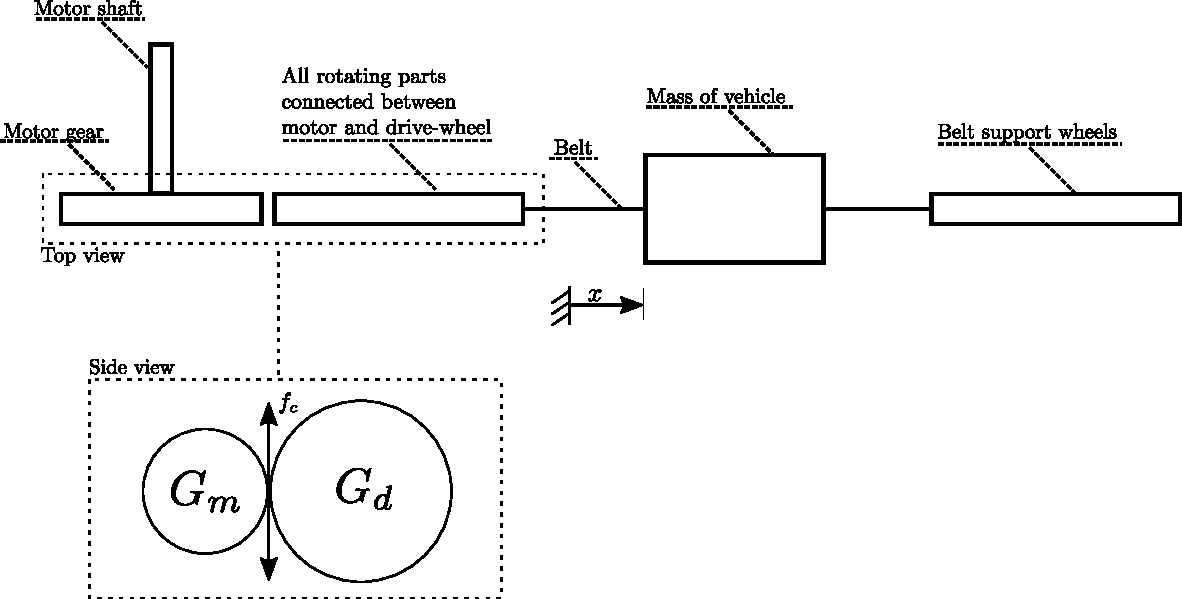
\includegraphics[scale=0.8]{figures/mechanicalDrawingSystem.pdf}
	\caption{A diagram showing the rough mechanical model of the drivetrain}
	\label{fig:DrivetrainMechanicalModel}
\end{figure}

% APPLICATION OF NEWTON'S SECOND LAW %

The derived torque from \eqref{eq:mechaUnloadedMotor} in \textit{motor modelling}, is extended with the contributions from the load, i.e. the drivetrain. A mechanical model of the gear, $G_m$, including the contributions from the motor shaft is illustrated in \figref{fig:MotorGearFreeBodyDiagram}.

\begin{figure}[H]
	\centering
	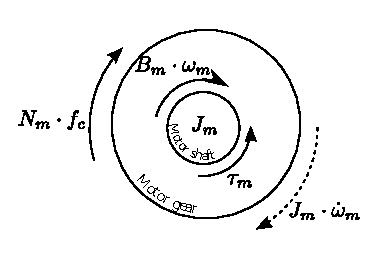
\includegraphics[scale=1.2]{figures/freeBodyMotorGear.pdf}
	\caption{A free body diagram of the motor gear}
	\label{fig:MotorGearFreeBodyDiagram}
\end{figure}

The contact force, $N_m \cdot f_c$, is a force which is opposite to the contact force on the gear, $G_d$, in \figref{fig:BlackBoxGearFreeBodyDiagram}, because of the rotations of the two gears. From \figref{fig:MotorGearFreeBodyDiagram}, the following equation can be extracted:
 
\begin{flalign}\centering
J_m \cdot \dot{\omega}_m(t) = \tau_m(t) - B_m \cdot \omega_m(t) - N_m \cdot f_c(t) 
\label{eq:MotorGearNewtonSecLaw}
\end{flalign}
\hspace{6mm} Where:\\
\begin{tabular}{p{1cm}ll}
& $J_m$ 			& is the motor's inertia [$kg \cdot m^2$] \\
& $\omega_m$        & is the angular velocity of the motor [$rad \cdot s^{-1}$] \\
& $\dot{\omega}_m$ 	& is the angular acceleration of the motor [$rad \cdot s^{-2}$] \\
& $\tau_m$ 		    & is the torque delivered by the motor [$N \cdot m$] \\
& $B_m$             & is the motor's friction coefficient [$N \cdot m \cdot s \cdot rad^{-1}$] \\
& $N_m$             & is the number of teeth on the gear ,$G_m$, connected to the motor shaft [$number\ of\ teeths$] \\
& $f_c \cdot N_m$	& is the contact force between the two gears [$N \cdot m \cdot number\ of\ teeths^{-1}$]
\end{tabular}

A mechanical model of the gear, $G_d$, is illustrated in \figref{fig:BlackBoxGearFreeBodyDiagram}.

\begin{figure}[H]
	\centering
	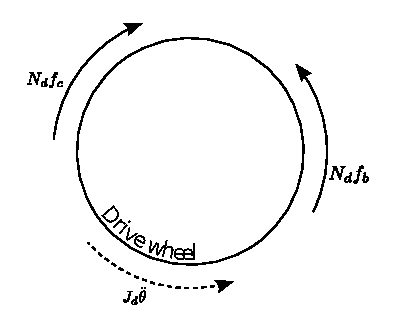
\includegraphics[scale=0.8]{figures/freeBodyDrive.pdf}
	\caption{A free body diagram of the `black box' gear}
	\label{fig:BlackBoxGearFreeBodyDiagram}
\end{figure}

The equation for \figref{fig:BlackBoxGearFreeBodyDiagram} is obtained the same way:
\begin{flalign}\centering
J_d \cdot \dot{\omega}_d(t) = N_d \cdot f_c(t) - N_d \cdot f_b(t)
\label{eq:BlackBoxGearNewtonSecLaw}
\end{flalign}
\hspace{6mm} Where:\\
\begin{tabular}{p{1cm}ll}
& $J_d$ 			      & is the `black box' gear inertia [$kg \cdot m^2$] \\
& $\omega_d$        & is the angular velocity of the `black box' gear [$rad \cdot s^{-1}$] \\
& $\dot{\omega}_d$ 	& is the angular acceleration of the `black box' gear [$rad \cdot s^{-2}$] \\
& $N_d$ 		     		& is the number of teeth on the `black box' gear [$number\ of\ teeth$] \\
& $f_b$             & is the coefficient of the contact force between $G_d$ and the belt [$N \cdot m \cdot number\ of\ teeths^{-1}$] \\
\end{tabular}

%% SSSECTION : BELT MODEL %%
\subsubsection{Belt Model}\label{BeltModel}

\begin{figure}[H]
	\centering
	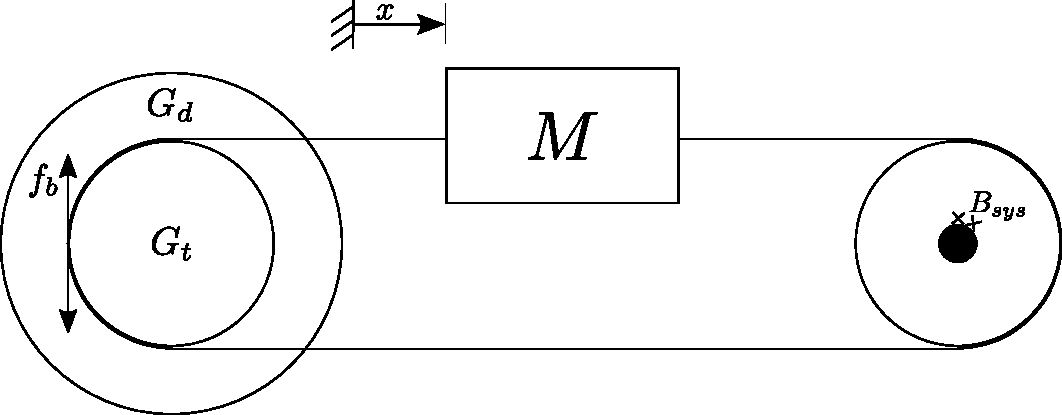
\includegraphics[scale=0.8]{figures/mechanicalDrawingBelt.pdf}
	\caption{A mechanical diagram of the belt part}
	\label{fig:BeltMechanicalDiagram}
\end{figure}

\begin{figure}[H]
	\centering
	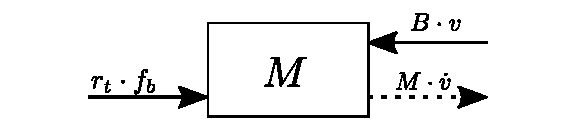
\includegraphics[scale=0.8]{figures/freeBodyBelt.pdf}
	\caption{A free body diagram of the belt driven mass}
	\label{fig:BeltFreeBodyDiagram}
\end{figure}

From \figref{fig:BeltFreeBodyDiagram}, the mechanical equation of the belt system on \figref{fig:BeltFreeBodyDiagram} is found to be:
\begin{flalign}\centering
M \cdot \dot{v}(t) = r_t \cdot f_b(t) - B_{sys} \cdot v(t)
\label{eq:BeltMassNewtonSecLaw}
\end{flalign}
\hspace{6mm} Where:\\
\begin{tabular}{p{1cm}ll}
& $M$ 			  & is the vehicle's total weight [$kg$] \\
& $v$        	& is the linear velocity of the behicle [$m \cdot s^{-1}$] \\
& $\dot{v}$ 	& is the linear acceleration of the vehicle [$m \cdot s^{-2}$] \\
& $r_t$ 		  & is the translational coefficient between the last gear and the belt [$m \cdot number\ of\ teeths^{-1}$] \\
& $B_{sys}$   & is the coefficient of the friction happening throughout the gears [$N \cdot s \cdot rad^{-1}$] \\
\end{tabular}

The assembling of a model for the drivetrain is made from these separate mechanical equations.

% SSSECTION : ASSEMBLING OF THE DIFFERENT EQUATIONS %
\subsubsection{Drivetrain modeling}\label{DrivetrainModeling}
The combination of \eqref{eq:MotorGearNewtonSecLaw}, \eqref{eq:BlackBoxGearNewtonSecLaw} and \eqref{eq:BeltMassNewtonSecLaw} makes it possible to get the linear velocity of the vehicle $v$ out of the torque $\tau_m$ given by the motor. Indeed, it is possible to link these equations throughout the contact force coefficients $f_c$ and $f_b$.\\\\
%
Taking the Laplace-transform of these equations helps arranging them and eventually, to find a transfer function from $\tau_m(s)$ to $V(s)$ :
%
\begin{flalign}\centering
J_m \cdot s \cdot \omega_m(s) = \tau_m(s) - B_m \cdot \omega_m(s) - N_m \cdot F_c(s) 
\label{eq:MotorGearNewtonSecLawLaplace}
\end{flalign}
%
\begin{flalign}\centering
J_d \cdot s \cdot \omega_d(s) = N_d \cdot F_c(s) - N_d \cdot F_b(s)
\label{eq:BlackBoxGearNewtonSecLawLaplace}
\end{flalign}
%
\begin{flalign}\centering
M \cdot s \cdot V(s) = r_t \cdot F_b(s) - B_{sys} \cdot V(s)
\label{eq:BeltMassNewtonSecLawLaplace}
\end{flalign}
%
By finding the expressions for $F_b$ from \eqref{eq:BeltMassNewtonSecLawLaplace} and then $F_c$ from \eqref{eq:BlackBoxGearNewtonSecLawLaplace}, it is then possible to insert $F_b$ expression into $F_c$'s and the latter into \eqref{eq:MotorGearNewtonSecLawLaplace}.
%
\begin{flalign}\centering
r_t \cdot F_b(s) =  M \cdot s \cdot V(s) - B_{sys} \cdot V(s) 
\label{eq:BeltContactForceLaplace}
\end{flalign} \todo{Get the second implication to be on the next line}
%
\begin{flalign}\centering
F_b(s) =  \frac{M \cdot s \cdot V(s) - B_{sys} \cdot V(s)}{r_t}
\label{eq:BeltContactForceLaplace}
\end{flalign} \todo{Get the second implication to be on the next line}

And $F_c$ is found this way from \eqref{eq:BlackBoxGearNewtonSecLawLaplace}:
\begin{flalign}\centering
N_d \cdot F_c(s) = J_d \cdot s \cdot \omega_d(s) + N_d \cdot F_b(s) 
\end{flalign}
\begin{flalign}\centering
F_c(s) =  \frac{J_d \cdot s \cdot \omega_d(s) + N_d \cdot F_b(s)}{N_d} =  \frac{J_d \cdot s}{N_d} \cdot \omega_d(s) + F_b(s)
\label{eq:GearsContactForceLaplace}
\end{flalign}

\todo{Get the steps to be on different lines}
%
Moreover, the relation of velocity for two gears $G_m$ and $G_d$ in contact is given by:
\begin{flalign}\centering
N_m \cdot \omega_m = N_d \cdot \omega_d, 
\label{eq:GearsVelocityRelation}
\end{flalign}

which is equivalent to :
\begin{flalign}\centering
\omega_m = \frac{N_d}{N_m} \cdot \omega_d \xRightarrow{\mathcal{L}} \omega_m(s) = \frac{N_d}{N_m} \cdot \omega_d(s).
\label{eq:BlackBoxGearNewtonSecLaw}
\end{flalign}
%
The same principle is applied from the angular velocity $\omega_d$ to the translational velocity $V$:
\begin{flalign}\centering
v(t) = r_t \cdot \omega_d(t) = r_t \cdot \frac{N_m}{N_d} \cdot \omega_m(t) \xRightarrow{} \omega_m(t) = \frac{N_d}{N_m \cdot r_t} \cdot v(t)
\label{eq:BlackBoxGearNewtonLaplaceNew}
\end{flalign}
Again, the Laplace transform is used to manipulate equations more easily:
\begin{flalign}\centering
\omega_m(s) = \frac{N_d}{N_m \cdot r_t} \cdot V(s).
\label{eq:BlackBoxGearNewtonLaplaceNew}
\end{flalign}

It is now possible to replace $\omega_d$ and $F_b$ in \eqref{eq:GearsContactForceLaplace}:
\begin{flalign}\centering
F_c(s) =  \frac{J_d \cdot s}{N_d} \cdot \frac{1}{r_t} \cdot V(s) + V(s) \cdot \left[\frac{M \cdot s + B_{sys}}{r_t}\right] = V(s) \cdot \left[\frac{J_d \cdot s}{r_t \cdot N_d} + \frac{M \cdot s + B_{sys}}{r_t} \right].
\label{eq:GearsContactForceLaplaceNew}
\end{flalign}

And the desired relation between the motor torque and the linear velocity is finally obtained :
\begin{flalign}\centering
\tau_m(s) = J_m \cdot \frac{N_d}{N_m \cdot r_t} \cdot V(s) \cdot s + B_m \cdot \frac{N_d}{N_m \cdot r_t} \cdot V(s) + N_m \cdot \left[\frac{J_d \cdot s}{r_t \cdot N_d} + \frac{M \cdot s + B_{sys}}{r_t} \right] \cdot V(s) = V(s) \cdot \frac{1}{r_t} \cdot \left[\frac{J_m \cdot N_d}{N_m} \cdot s + N_m \cdot J_d \cdot s + M \cdot s + N_m \cdot B_{sys} + B_m \cdot \frac{N_d}{N_m} \right]
\end{flalign}

Therefore, the transfer function from $\tau_m$ to $V$ is :
\begin{flalign}\centering
\frac{V(s)}{\tau_m(s)} = \frac{r_t}{\left[\frac{J_m \cdot N_d}{N_m} + N_m \cdot J_d + M\right] \cdot s + \left[B_{sys} \cdot N_m + B_m \cdot \frac{N_d}{N_m} \right]}
\label{eq:TransferFunctionTorqueToVelocity}
\end{flalign}

Eventually, it is possible to draw a block diagram for the drivetrain, from the motor torque to the vehicle's velocity with \eqref{eq:TransferFunctionTorqueToVelocity} and also back to the angular velocity with \eqref{eq:BlackBoxGearNewtonLaplaceNew}, see \figref{fig:BeltFreeBodyDiagram}.

\begin{figure}[H]
	\centering
	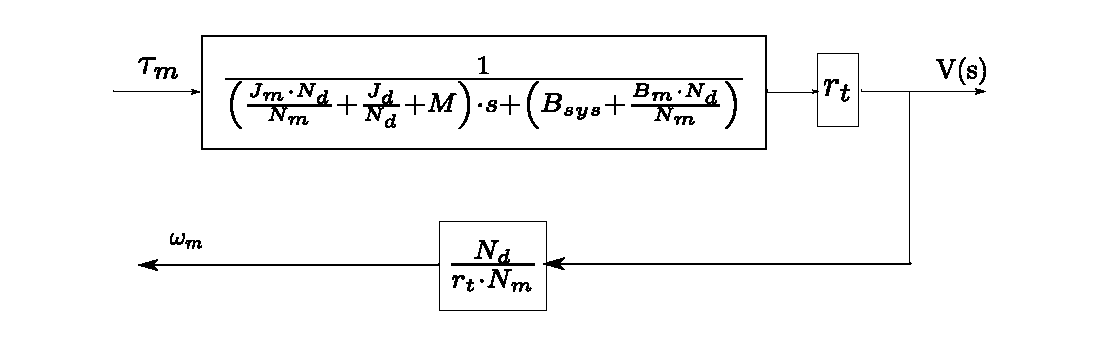
\includegraphics[scale=0.8]{figures/blockDiagramDrivetrain.pdf}
	\caption{A block diagram of the drivetrain}
	\label{fig:BlockDiagramDrivetrain}
\end{figure}
